\newpage
\section{Context}
This first section of the report aims at providing to the reader a complete overview of the background of the CHIC project itself. In this section, we present our team, interdisciplinary work and an overview of the Toygether plush toy as designed with our whole team. 

\subsection{Team description}
As part of the CHIC, the project is strongly grounded in an interdisciplinary environment. Unlike "usual" engineering projects developed at EPFL, our work has been accomplished in close interaction with designers and business students. Such diversity within the team evokes a unique approach to the development process. 

\medskip
The team composition is illustrated in the following list. Students have been selected from the three "Haute Ecoles" of Lausanne: the École Cantonale d'Art de Lausanne (ECAL), the École Polytechnique Fédérale de Lausanne (EPFL) and the Université de Lausanne (UNIL).

\vspace{1cm}
\begin{tabular}{m{2cm}m{5cm}m{2cm}m{5cm}}
    
    
\includegraphics[width=2cm]{images/icon_marjane.png} & \textbf{Marjane Amara} \newline Industrial Design &
    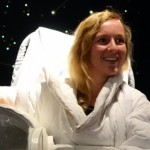
\includegraphics[width=2cm]{images/icon_chloe.jpg} & \textbf{Chloe Dickson} \newline Firmware Engineering \newline Mechanical Engineering \\
    
     & & & \\
    
    
\includegraphics[width=2cm]{images/icon_estelle.jpg} & \textbf{Estelle Geneux} \newline Business &
    
\includegraphics[width=2cm]{images/icon_yann.jpg} & \textbf{Matteo Yann Feo} \newline Software Engineering \\
    
     & & & \\
    
    
\includegraphics[width=2cm]{images/icon_simone.png} & \textbf{Simone Sanso} \newline Electronic Engineering \newline Firmware Engineering &
    
\includegraphics[width=2cm]{images/icon_luca.png} & \textbf{Luca Sassoli de Bianchi} \newline User Experience\\
\end{tabular}

\subsection{Product description}
\label{sec:product_Description}

Our product, named Toygether, is a connected plush toy that enables children to play with their parents, even when far away. The plush toy is screen-less and the electronics are hidden, allowing the parents to stay in contact with their kids, without having to rely on too present screens. In order to showcase the end result of the development to both investors and potential customers, Simone, Estelle and Luca worked on our descriptive one-pager (see figure \ref{fig:one_pager} on the upcoming page).

\begin{figure}[hbtp]
    \centering
    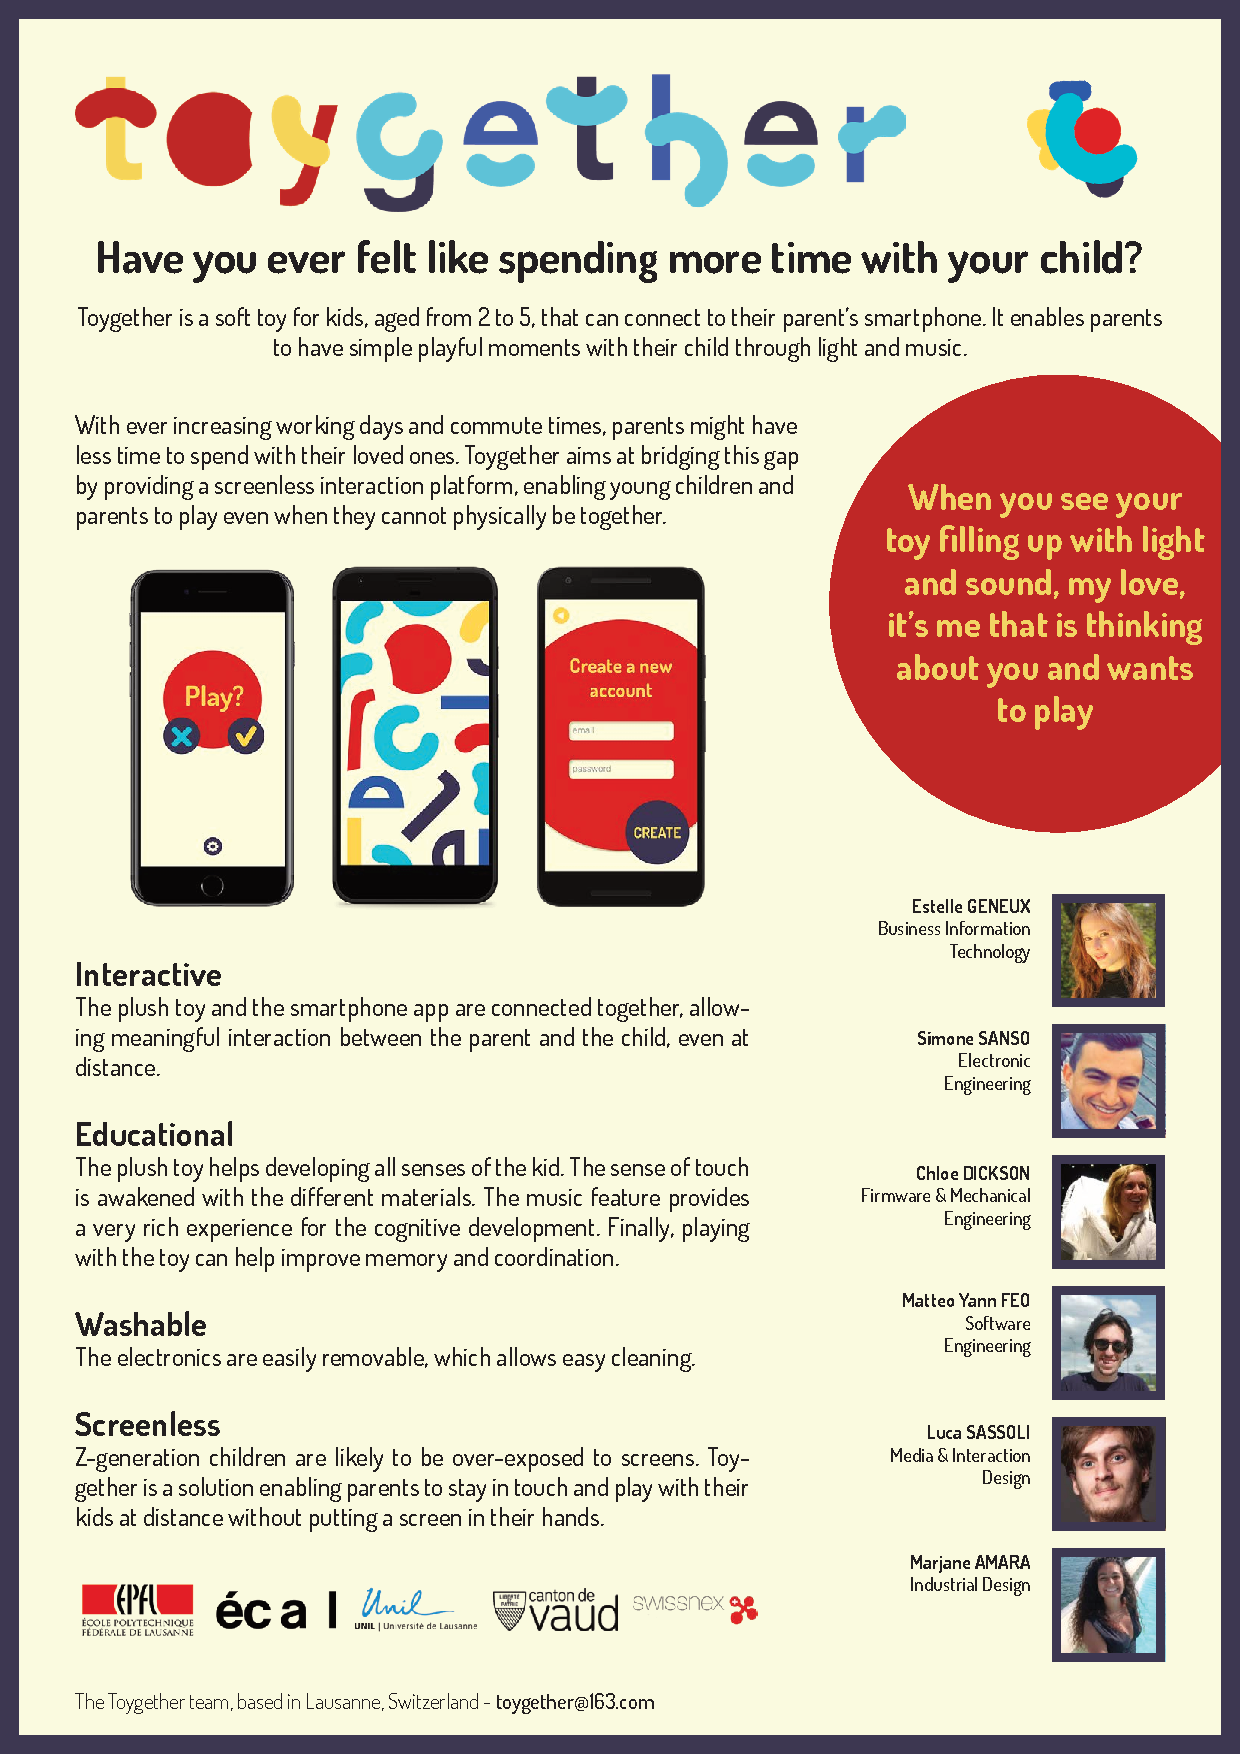
\includegraphics[scale=0.78]{images/intro_one_pager.pdf}
    \caption{Descriptive one-pager about Toygether}
    \label{fig:one_pager}
\end{figure}

\medskip
Finally, the description of the project has also been proposed on a landing-page. This web-page \cite{toygether_web} has been built with Yann's support in order to give a direct access on the developed result to anyone interested in learning about the project.

\newpage
\subsection{Work with ECAL designers}

\subsubsection{Industrial Design}
Marjane, our industrial designer, was in charge of designing the "soft" part of the plush toy and the housing for the electronics (or "blackbox"). Chloe collaborated with her for the design of the soft electronics (or "soft PCB") and for ensuring that her design was always compatible with engineering possibilities. 

\vspace{1cm}
\begin{figure}[ht]
    \centering
    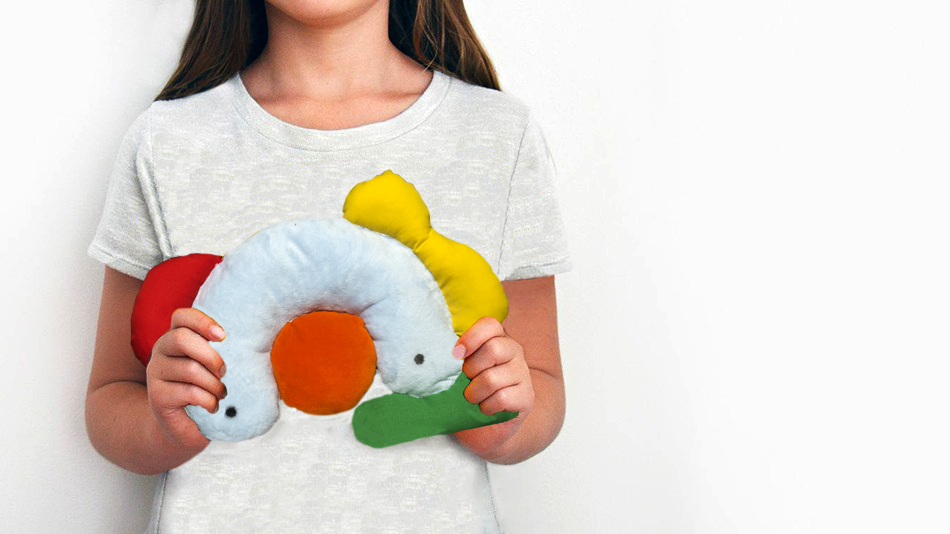
\includegraphics[scale=0.38]{images/kid_toygether.jpg}
    \caption{Plush toy presented at MS5, with no visible electronics}
    \label{fig:kid}
\end{figure}
Our main challenge with the industrial design was to ensure that the plush toy shape always stayed compatible with what was possible to manufacture on the engineering side, in particular with respect to size, shape and connectivity of the electronics. 

\paragraph{Iterations} The first ideas for the shape of our plush toy were animal-like toys. As we were developing a health-tracker, we wanted the toy to be friendly and look like a "companion" to the child's daily life. The first prototype we presented at MS4 was a little monster (Fig. \ref{fig:monster}), which children liked a lot, but which did not "need" electronics inside and identified with a "Disney" character, rather than having its own unique identity.

\medskip We then pivoted to an interactive and playful plush toy with multiple soft sensors instead of an activity tracking plush toy. For the next milestones, Marjane came up with a plush toy made up of abstract shapes (Fig. \ref{fig:iterations}), which call to the child's imagination and are completed by the electronics inside. The large and distinguishable zones each conceal a soft touch sensor and an interactive play zone, with a LED and an associated sound. Marjane also played on textures and colours, to make the plush toy more appealing to toddlers, even when offline. 

\begin{figure}[H]
    \centering
    \subfloat[First iteration of the plush toy\label{fig:monster}]{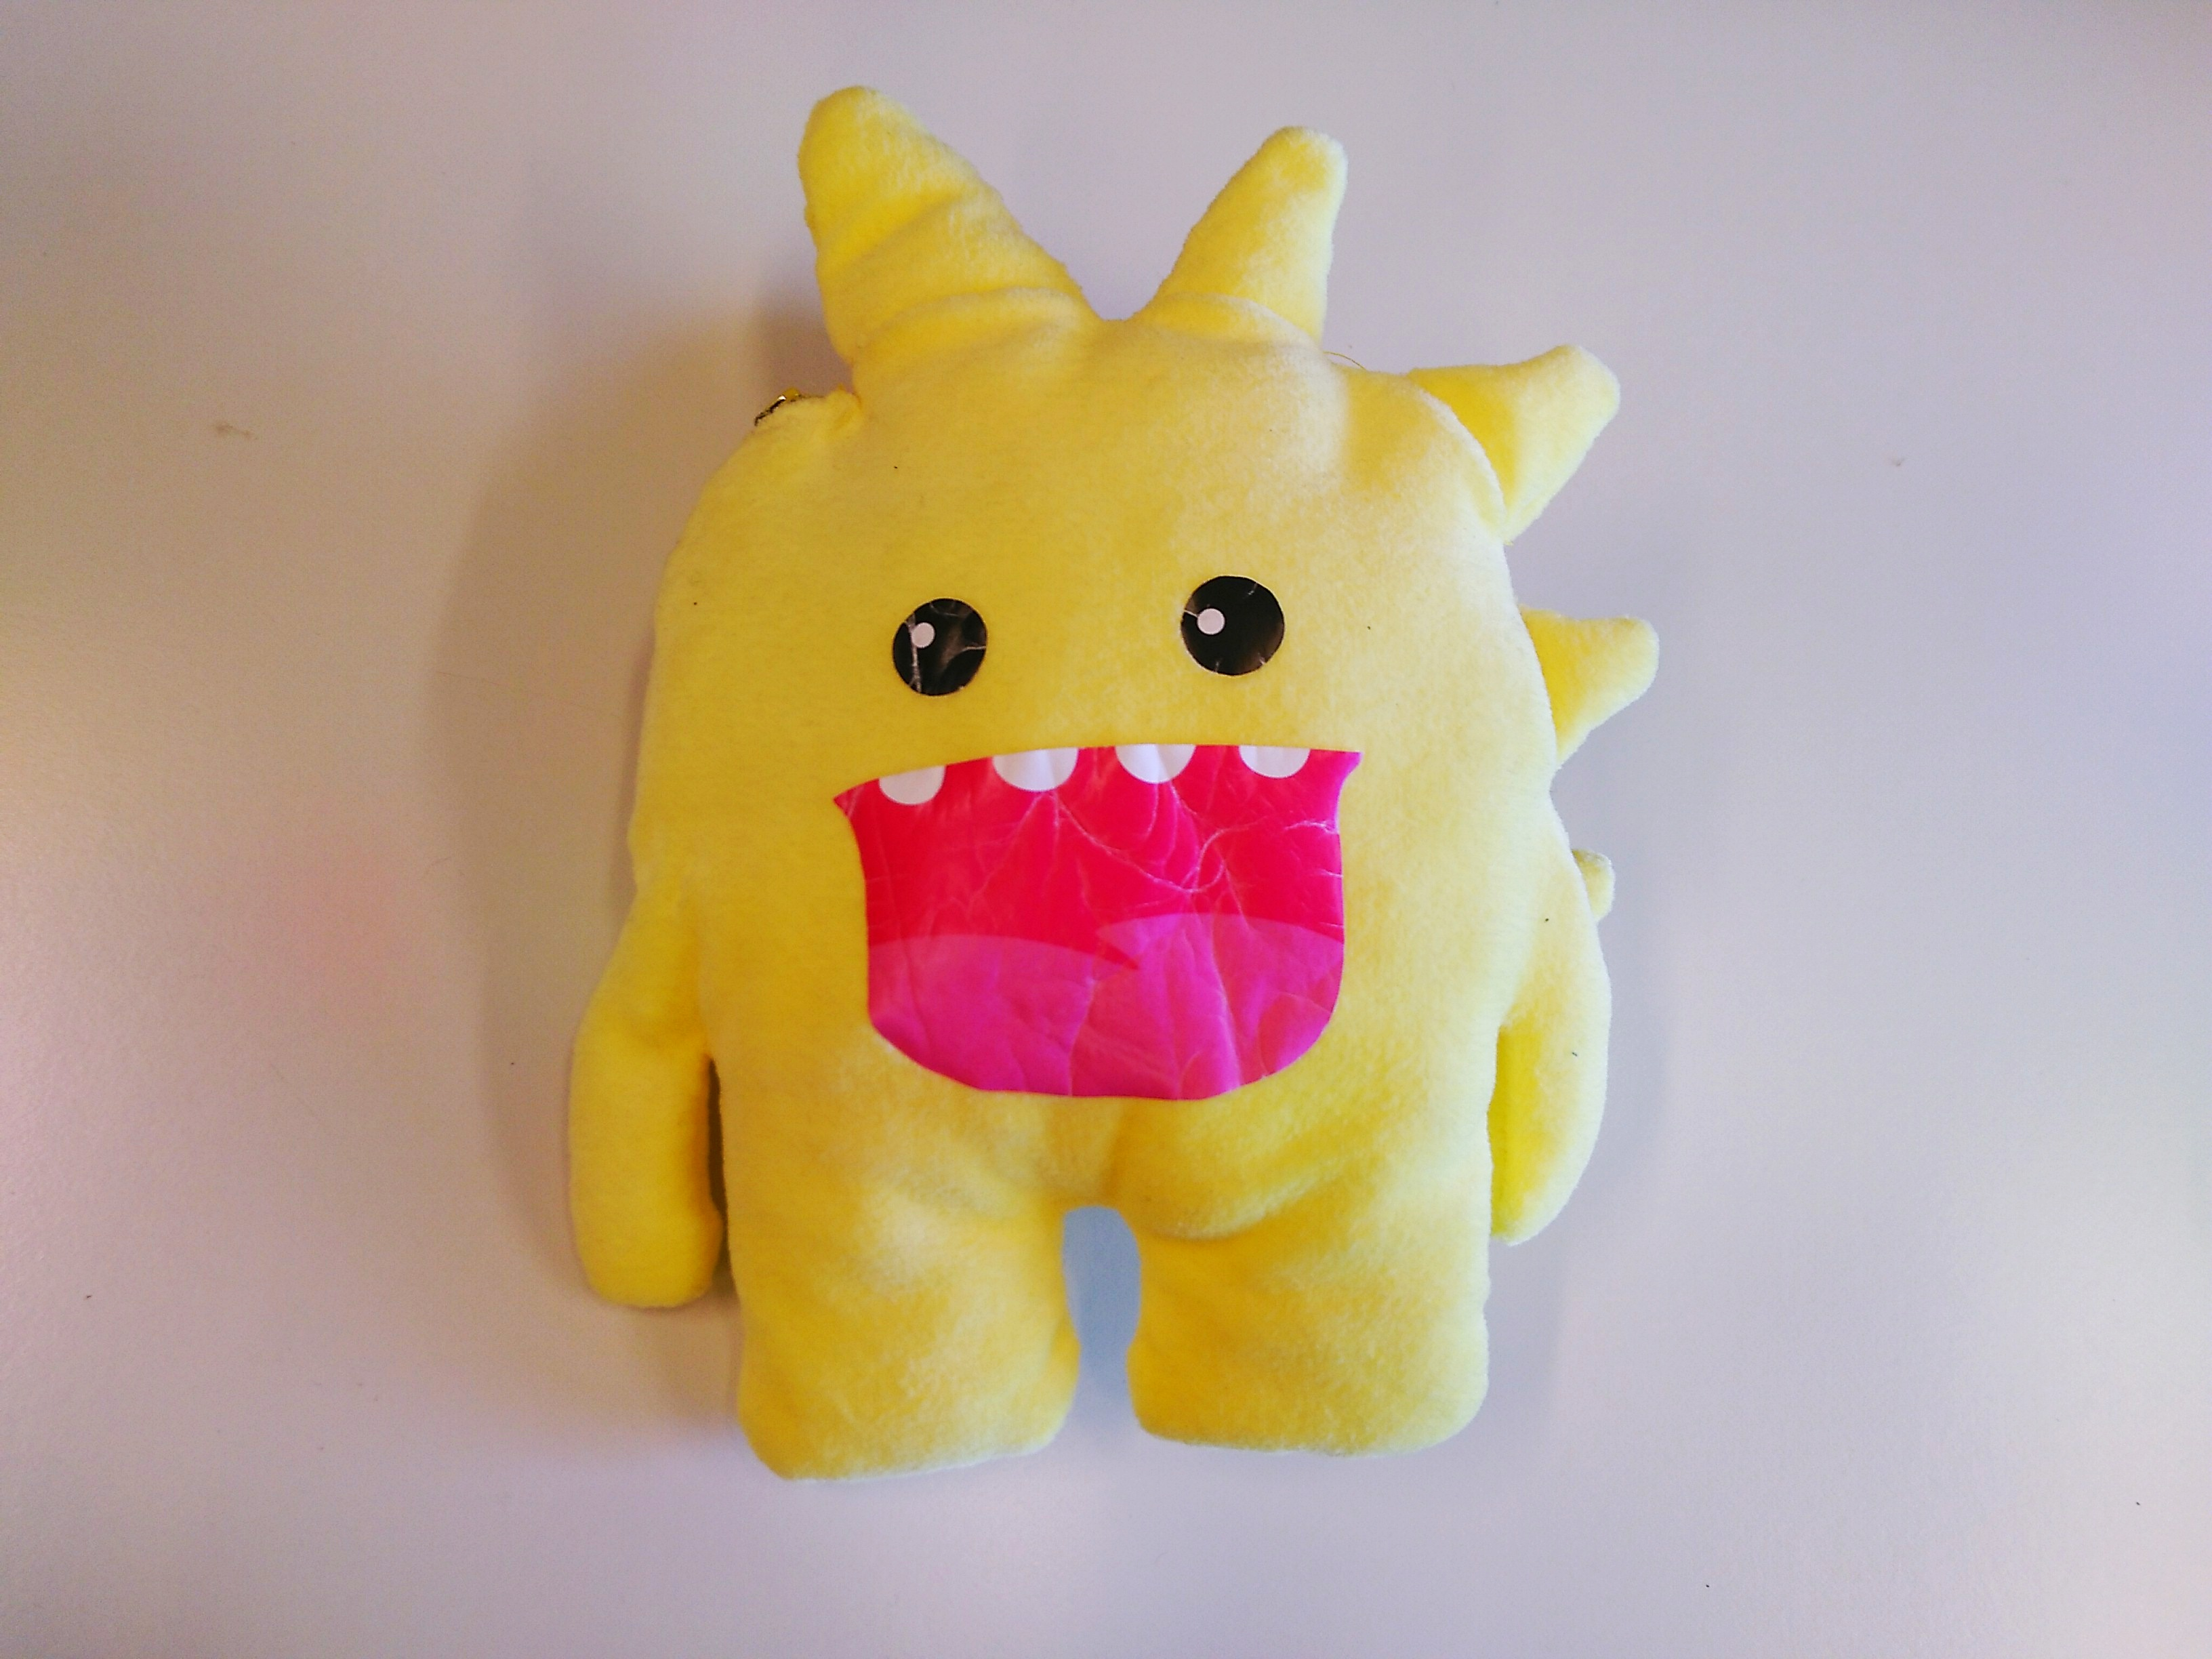
\includegraphics[width=0.3\textwidth]{images/monster.jpg}}\hfill
    \subfloat[Design brainstorming for MS4\label{fig:iterations}] {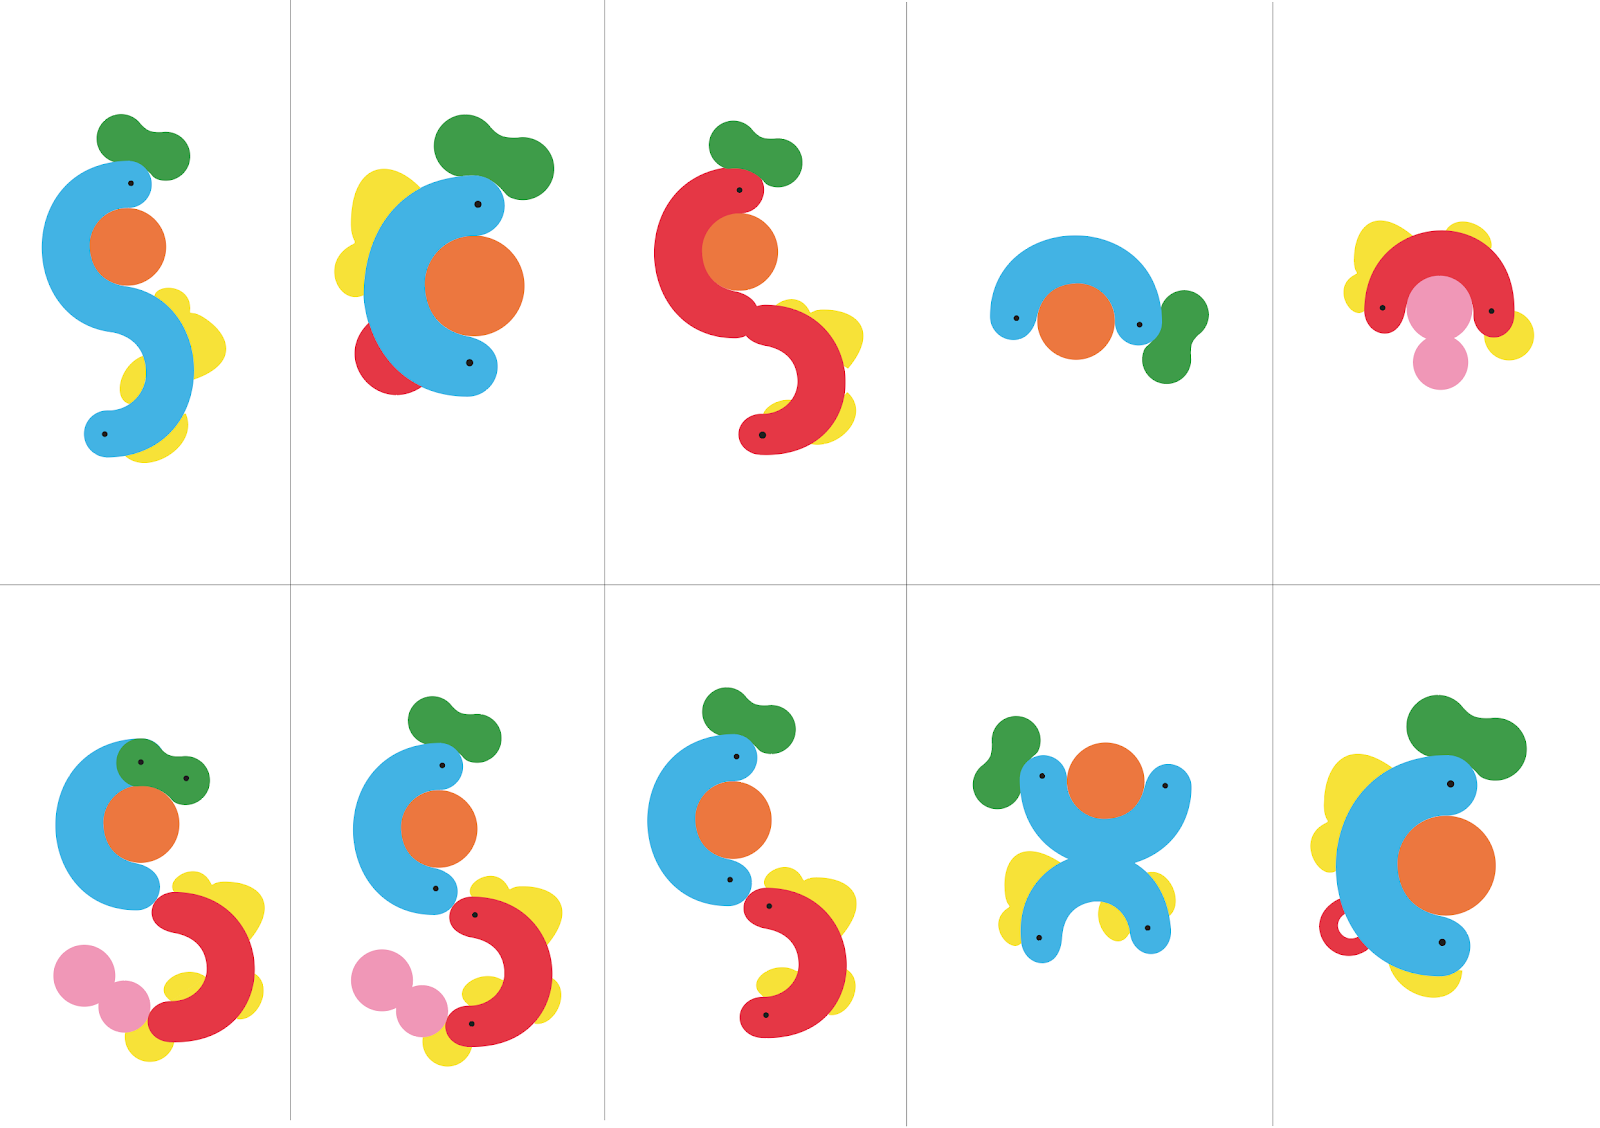
\includegraphics[width=0.35\textwidth]{images/iterations.png}}\hfill
    \subfloat[Plush toy presented at MS5\label{fig:ms5}] {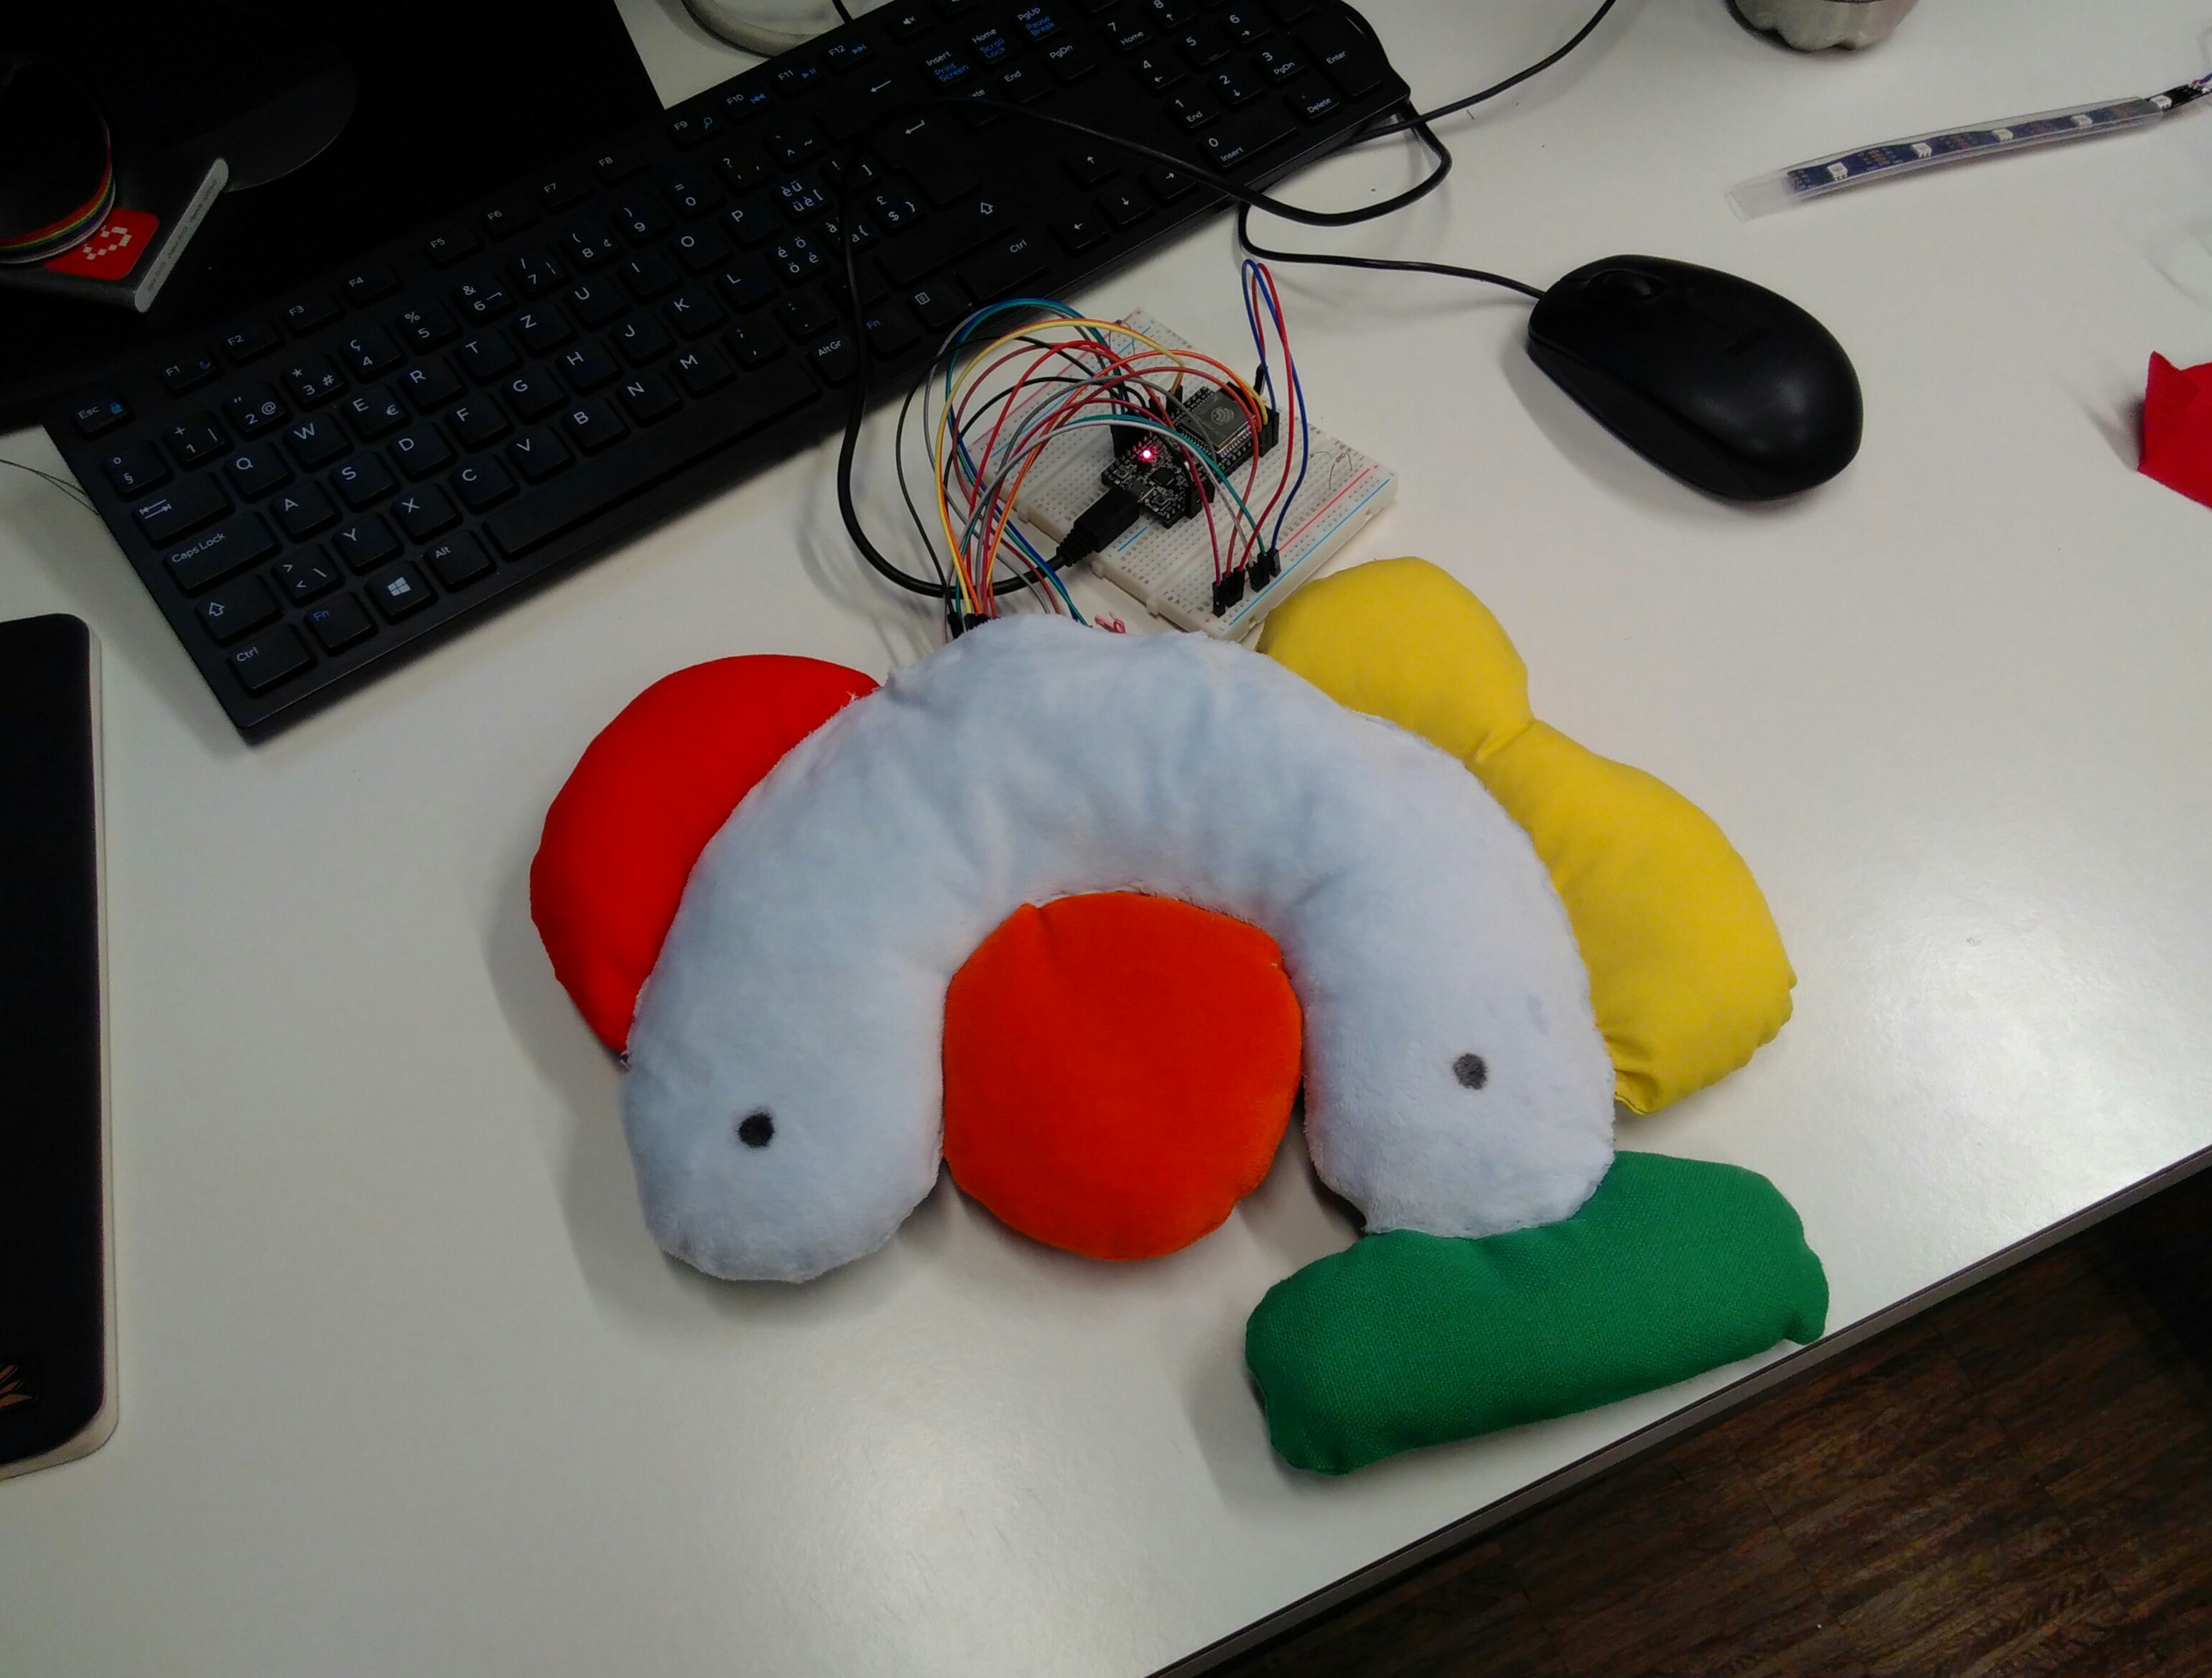
\includegraphics[width=0.3\textwidth]{images/ms5.jpg}}\hfill
    \caption{Design iterations for the plush toy} 
    \label{fig:industrial_design}
\end{figure}


For the design of the plush toy, we had to define some restrictions, according to engineering resources and possibilities. These were: 

\begin{description} [align=left]
    \item [Size of the main body] The plush toy needed to have a space of at least $3\times7\times5$ centimetres in order to fit the blackbox with the PCB and battery.
    \item[Shape of the plush toy] The plush toy needed to hold a "soft PCB" (described in Section \ref{sec:softPCB}), with textile conductors and sensors. For ease of manufacturing and electronics embedding, the plush toy was designed in "2.5D", that is, the sewing pattern had to be in 2D and the plush toy gets its shape with the stuffing but still remains "flat". The soft PCB also had to be easily inserted in the plush skin, limiting futher the design of the plush shape.
    \item[Blackbox] The blackbox needed to hold the PCB and battery, while giving access to connectors for the soft PCB. This means that the blackbox needed some openings for connectivity and user manipulations.
    \item[Washability] We wanted the blackbox to be removable, meaning that the connectors between hard and soft PCB had to be user-friendly and as simple as possible. The soft electronics also need to be robust to washing.
\end{description}

\subsubsection{Media and Interaction Design}
\label{sec:interaction_design}

The media \& interaction designer of the team, Luca, has been working on the user-experience of the project. While he has been collaborating with Marjane on the shape, his main focus was designing the child-parent game interaction and experience while using the product. Luca was also in charge of graphic design and defining our brand identity. Moreover, he has been working closely with Yann, the software engineer, in order to design the Android app for parents.

\medskip
The final output of the collaboration is a series of user-focused behavioural descriptions that he/she would experience during the interactions. The work covered the whole user experience of both parent and child, from the very first sing-up and pairing to the play session itself. In the next page, we will illustrate this latter element in detail in order to give to the reader a more concrete overview on the usage of the product before dealing with engineering details.

\begin{figure}[H]
    \centering
    \subfloat[\label{fig:interaction1}]{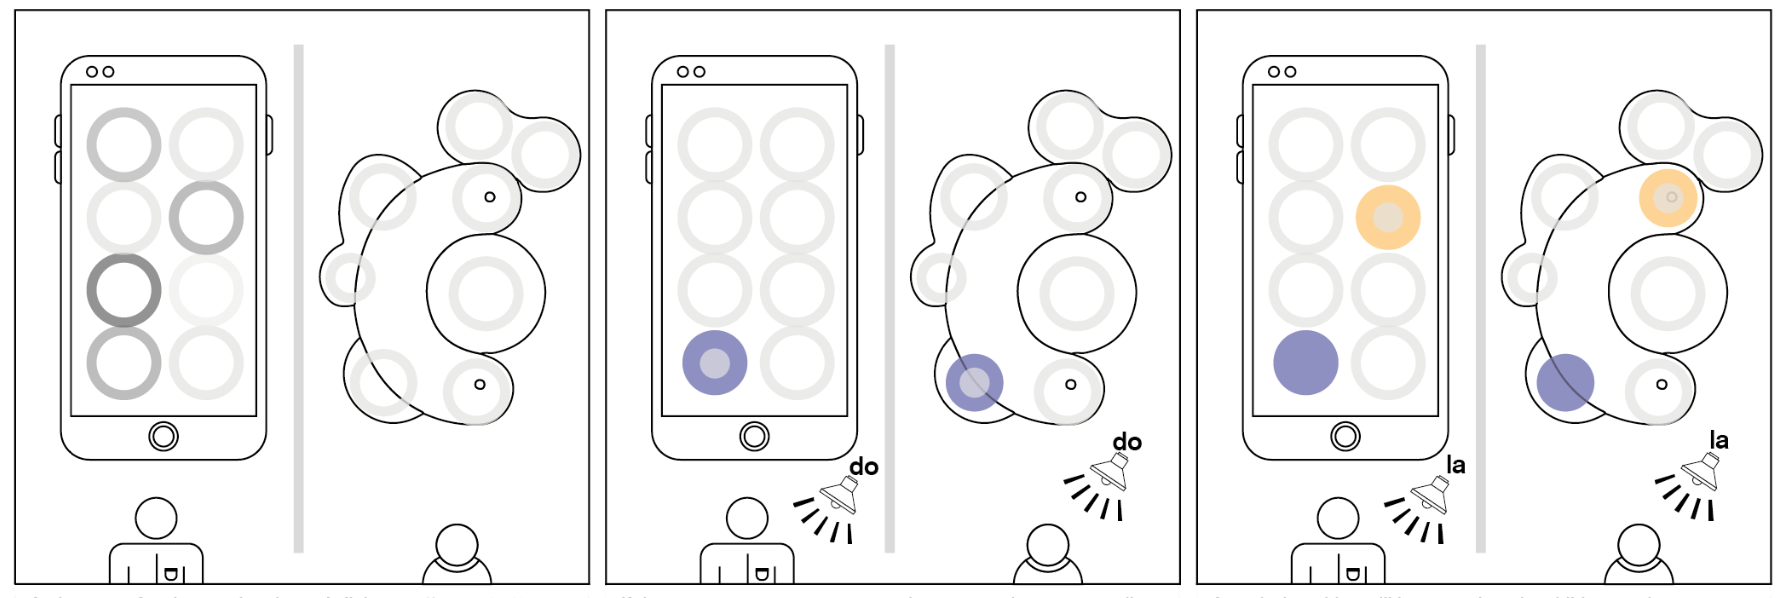
\includegraphics[scale=0.35]{images/FW/play_1.png}}\hfill
    \subfloat[\label{fig:interaction2}] {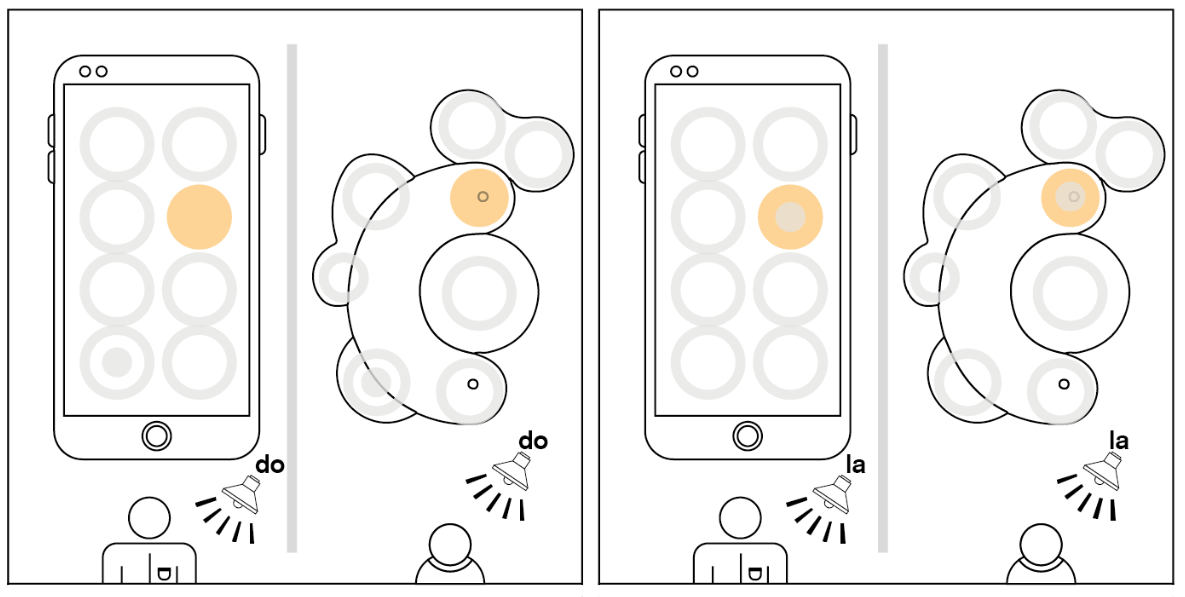
\includegraphics[scale=0.35]{images/FW/play_2.png}}\hfill
    \caption{Interaction design for child/parent game session } 
    \label{fig:game_id}
\end{figure}

\medskip
Figures \ref{fig:interaction1} and \ref{fig:interaction2} illustrate a sequence of interactions between child and parent. At the very start of the play session (first square of figure \ref{fig:interaction1}), all LEDs of the plush toy are turned off and the parent application is filled with eight grey areas. When the parent interacts with one of those zones on the app, the corresponding LED on the plush toy will turn on with the parent's colour (blue, for instance). At the same time, a musical note will be played on both sides of the interactive session (i.e. parent and child). The musical notes are assigned to each of the 8 zones in order to complete a full octave. An equivalent result happens whenever the child interacts with touch sensors of the plush toy: the corresponding area on the parent app is turned on with the child's colour (orange, for instance) and the musical note is played in the background. Figure \ref{fig:interaction2} illustrates the behaviour of the interaction, whenever someone presses a zone that has been previously turned on. In the first frame, the child pressed on the blue zone that the parent turned on previously, which will cause the corresponding musical note to play again, before having the zone turning off. The last frame showcases the visual responses, whenever someone presses on their own zone (i.e. the child pressing again on the orange zone she has previously turned on): the corresponding musical note will be played again in the background, while the colour blinks without turning off. In fact, only the opposite player of the session can turn off zones of the first player.%, which pushes for non-stop series of interactions while playing together.

\subsubsection{Visual Identity}

\begin{figure}[H]
    \centering
    \subfloat[Initial logo design tentative\label{fig:logo_old}]{
\includegraphics[scale=0.95]{images/logo_old.png}}\hfill
    \subfloat[Final logo design\label{fig:logo_new}] {
\includegraphics[scale=0.2]{images/logo_new.png}}\hfill
    \caption{Successive design iterations for brand and visual identity } 
    \label{fig:logo}
\end{figure}

\medskip
The work that Luca accomplished with us during the last semester has also been to define a complete visual identity of the product and brand we were developing. Figure \ref{fig:logo} illustrates the iterations of the brand's logo. Thanks to the interdisciplinary dimension of the CHIC project, one can understand that evaluations and advancements are not only present in engineering aspects of the project (as we will later report), but also in both the form and the identity of the latter. The final visual identity of the \textit{Toygether} brand has been inspired by the shape of the toy from the industrial design work, as illustrated in Figure \ref{fig:industrial_design}. The Android app illustrated at the end of the report (see subsection \ref{subsec:android}) will strongly be influenced by the visual identity, in particular in the parent's phone app graphical user interface.

\subsection{Business analysis}

Estelle, student of the Business School HEC (Haute Ecole de Commerce) from UNIL, collaborated on the ideation of the project during the first semester, then focused on the economical, business and marketing aspects of the project during the second semester. 

\medskip Some of Estelle's work on the business side also determined features for the engineers. For example, we wanted the plush toy to symbolise the connection with one parent (as opposed to several people). On the business side, this means more sales if people want plush toys connecting the child with several caretakers, and on the engineering side it determines some of the interaction features on the app and plush toy. For the design, it could drive us to imagine several different shapes to design a full plush toy collection.

%\medskip Lastly, the "elevator pitch" of the product was also handled by Estelle, who knows very well how to catch the attention of the listeners as seen for the development of the one-pager. 

\newpage

\begin{table}[]
\centering
\caption{Cost break-down for the outside skin production}
\label{tab:cost-skin}
\begin{tabular}{l|p{4.5cm}||p{4.5cm}|}
\hline
\multicolumn{1}{|l|}{\textbf{Plush}}                           & \textbf{Quantity per plush toy}        & \textbf{Price per plush toy(chf)} \\ \hline \hline
\multicolumn{1}{|l|}{Tissus normal}                            & 6 pieces 30x30                                               & 2.4                               \\ \hline
\multicolumn{1}{|l|}{Fermeture éclair}                         & 10cm                                                         & 0.025                              \\ \hline
\multicolumn{1}{|l|}{Rembourrage anti-acariens} & 70g                                                          & 0.85                              \\ \hline
\multicolumn{1}{|l|}{Raw Materials}                            &                                                              & 3.275                              \\ \hline
\multicolumn{1}{|l|}{CTM}                                      & cutting, sewing, machining, pressing, examination, filling & 3.684                       \\ \hline
\multicolumn{1}{|l|}{Production}                               & Per plush                                                    & 6.959                       \\ \hline
\multicolumn{1}{|l|}{Shipping}                                 & Per plush                                                    & 1.044                       \\ \hline
\multicolumn{1}{|l|}{Duty}                                     & Per plush                                                    & 0.557                         \\ \hline
                                                               & \textbf{TOTAL}                                  & \textbf{8.56} \\ \cline{2-3} 
\end{tabular}
\end{table}

\begin{table}[]
\centering
\caption{Cost break-down for the "blackbox" production}
\label{tab:cost-blackbox}
\begin{tabular}{l|p{4.5cm}||p{4.5cm}|}
\hline
\multicolumn{1}{|l|}{\textbf{Black box}}      & \textbf{Quantity per plush toy} & \textbf{Price per plush toy (chf)} \\ \hline \hline
\multicolumn{1}{|l|}{Leds}                    & 9                             & 2.7                             \\ \hline
\multicolumn{1}{|l|}{Tissus + fil conducteur} & 1.5m + 225cm2                 & 1.2                              \\ \hline
\multicolumn{1}{|l|}{Speaker}                 & 1pc                           & 1                                \\ \hline
\multicolumn{1}{|l|}{PCB Components}          & See Bill of materials         & 12.17                            \\ \hline
\multicolumn{1}{|l|}{PCB}                     & 1pc                           & 0.35                             \\ \hline
\multicolumn{1}{|l|}{Charger}                 & 1pc                           & 1.3                              \\ \hline
                                              & \textbf{TOTAL}                & \textbf{18.72}                  \\ \cline{2-3} 
\end{tabular}
\end{table}

\begin{table}[]
\centering
\caption{Cost break-down for variable overheads of the production}
\label{tab:cost-extra}
\begin{tabular}{|l|p{4.8cm}|}
\hline
\textbf{Other variable costs}      & \textbf{Price per plush toy (chf)} \\ \hline \hline
Warehouse workers                  & 0.6                                \\ \hline
Package price                      & 0.07                               \\ \hline
Marketing and other overhead costs & 1.5                                \\ \hline
Packing                            & 0.4                                \\ \hline
Shipping                           & 1.5                                \\ \hline
\textbf{TOTAL}                     & \textbf{4.07}                      \\ \hline
\end{tabular}
\end{table}

\clearpage

\newpage

\medskip By conducting several interviews and by understanding the type of customer that could be interested in the product, pricing strategies have been deduced. Thanks to the work conducted with the engineers, it has been to develop a total fabrication cost of approximately 30 CHF per unit expectation. The cost has been computed taking into account selected components that will be later on illustrated in details. Tables \ref{tab:cost-skin}, \ref{tab:cost-blackbox} and \ref{tab:cost-extra} on the previous page illustrate a clear break-down of each overhead present during the production of specific parts. In order to take into account development costs of R\&D and marketing, the retail price has been fixed to 59.90 CHF. 

\subsection{SHS research project and insights}

As part of the minor \textit{Science, Technology and Area Studies (STAS)} chaperoning the CHIC program, Simone and Yann enriched the contextualisation of the development within the Chinese reality with a parallel research project on social contexts. The latter has been conducted during the Spring semester under the guidance of Mr. Laperrouza. The aim of the research project has been to investigate, with more social and social sciences perspectives, how our project - a connected plush toy for distant families - would fit within the Chinese context. 

\medskip
The final work mainly focused on the extensive reality of so-called left behind children in rural China. According to previous studies on the topic, 80\% of migrant workers leave their children "behind" in their home-village. Those parents are often obliged to reach more urbanised areas in order to increase the remittances sent to their families, while children are raised in the rural village by their grandparents or, in some cases, without anyone taking care of them. During our research, we have been able to show how such situation has been proved to raise education standards for the children, who, thanks to increased remittances from their migrant parents, have better access to health and academic services. On the other hand, strong negative implications on the children mental well-being have been identified, which could increase the risks of depression.

\medskip
In accordance with the CHIC project, we questioned if the adoption of communications technologies like, but not limited to, our connected plush toy, could benefit left-behind children. The research was enriched by a "fieldwork" conducted in Switzerland, in order to estimate the importance for distant families to communicate and, more particularly, for children of a young age. The results have been extremely encouraging on pursuing the development of the plush toy, as we obtained important insights on the crucial family bond that young children build with their parents through communication technologies. 